\section{Findings}
\label{sec:result}
\subsection{Primary Evaluation}

The first set of findings came directly from the testing performed by the authors. Initially, we found two problems regarding login and setting up a new account. While registering for the first time with an official departmental email (with .buet.ac.bd as the suffix), the input form showed an error. As it turned out, we could not proceed because some of the input fields got frozen. Changing the email input field to a regular email address solved this issue. Next while trying to perform a login, the website took an unusually high amount of time on average. 

To start with the web pages, we first landed on the homepage and navigated around it. It contained 7 header tabs constantly being displayed at the top of the webpage. Moving downwards, there were notice and news sections that contained hyperlinks to the latest notices sorted from the newest to the oldest order. There was a video demonstrating the history of passports and e-Passports in the country. There were also video links to e-Gate demonstrations.
Finally, there were 3 important additional links that direct to FAQs, About us, and Feedback pages. The FAQ page looked well-organized with multiple sections that answer some questions related together. The About us page provided a link to the website of the Department of Passport and Immigration. The feedback section, last updated on March 14, 2022, contained a link to the feedback form under the midterm evaluation of the whole project that asked for thoughtful feedback from the users to better improve the project.

Then we navigated through the tab titled ‘5 steps to e-Passport’ that enlists a brief set of necessary instructions in a step-by-step fashion. All the active 4 links were working fine, and the hyperlinks were marked differently for a better visual experience. The link from ‘Step 4’, listing the necessary documents to take with a user for biometric enrolment, had some information gap issues inside. Some contents of the document list were not clear enough. For example, it just mentioned one needs to bring NID and/or other identification documents. But in reality, one discovers that he/she needed to carry both original copies and photocopies of that document, after going to the passport office. The same problem was faced in the case of any previous passport, there was not anywhere mentioned on the website about bringing photocopies. This information should have been present in the system beforehand to improve user experience.

The information presented in the ‘Urgent Application’ tab looked quite well-organized and clear. There was a separate ‘Instructions’ tab that present important dos and don’ts regarding the application form. But it would have been better if those instructions were found alongside the application form itself. The ‘Passport fee’ tab contained information about different categories of passport fees based on different validity duration, total pages, and delivery types. 

There remained 3 major sections of the website that we, the authors could not check and verify till the exact end, as it required us to create and fill up a completely new application again from the scratch, while we already had our own passports registered. These sections are the Application Form, Check Status, and Contact tabs. Hence, we had to depend on the user feedback for these sections to better understand the upsides and downsides of the system. contact section provided a series of drop-down menus to select the category of query one is looking for.

\begin{figure}[ht]
\centering
\centerline{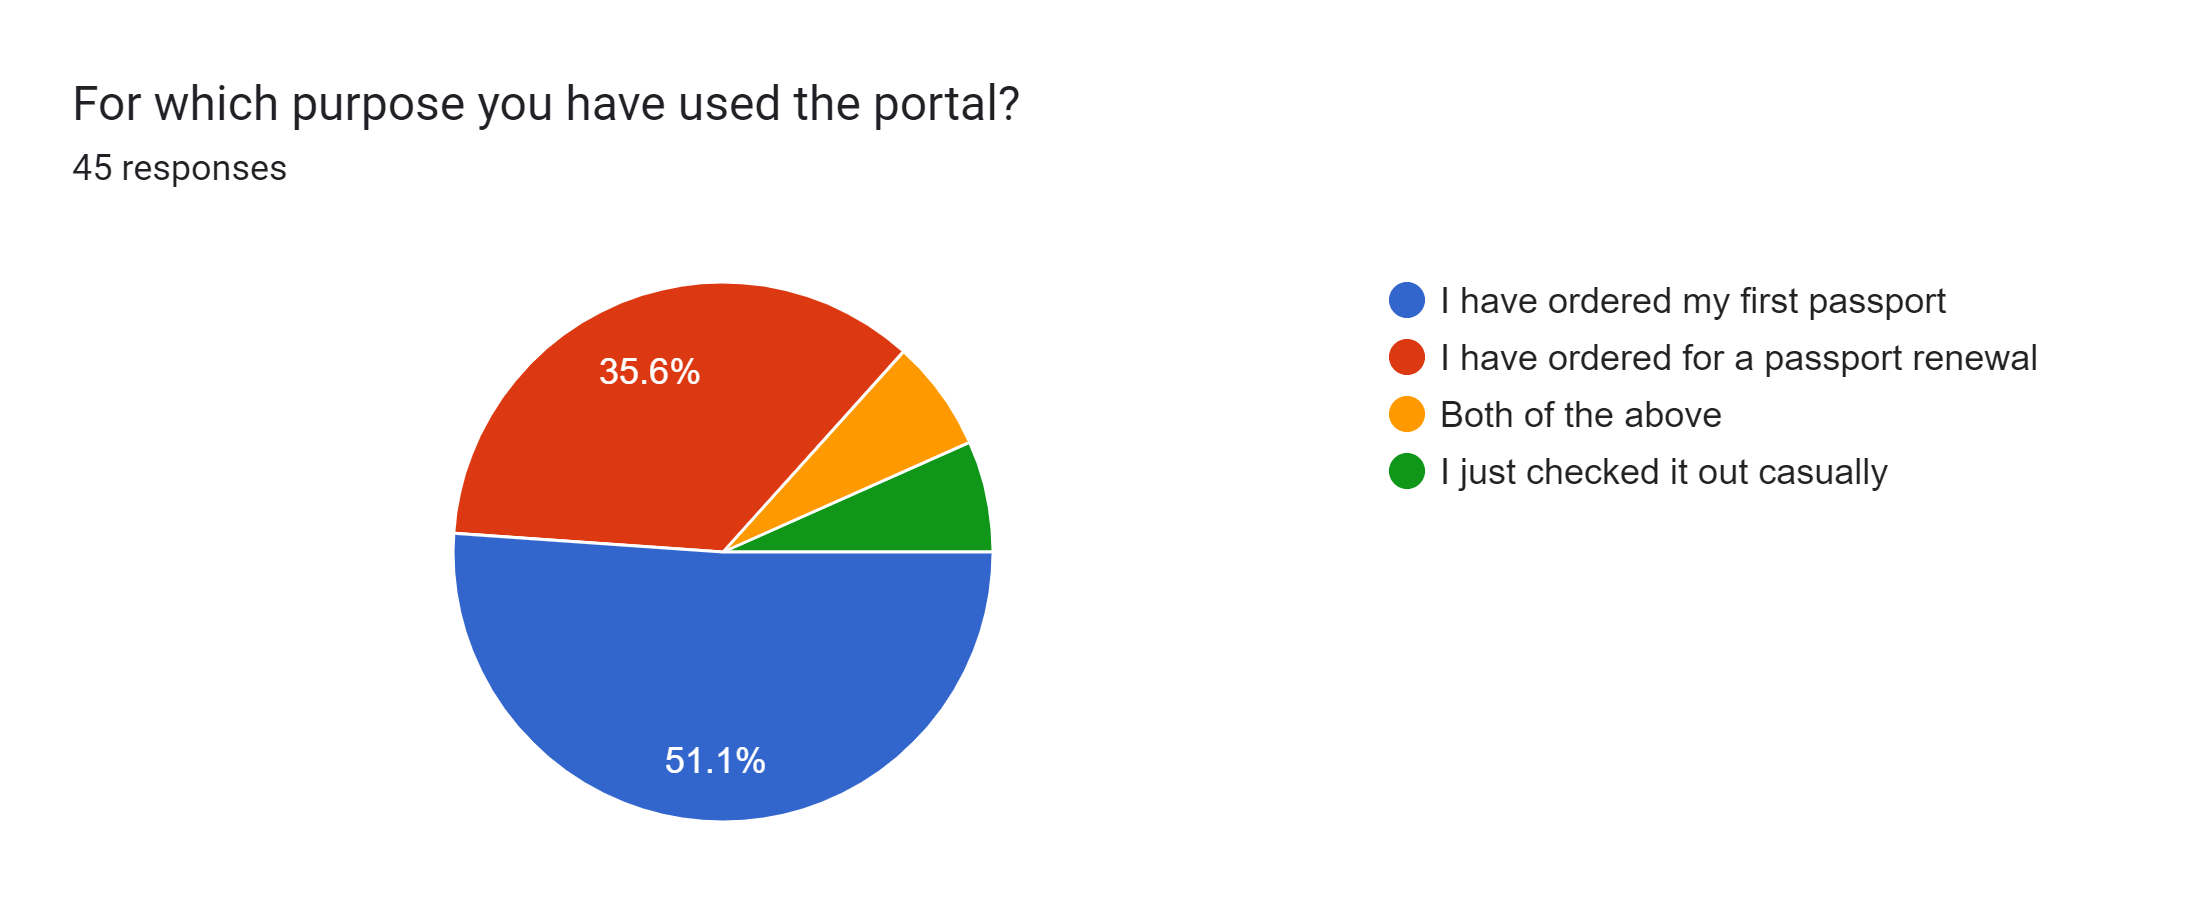
\includegraphics[width=\linewidth]{Figures/purpose.png}}
\vspace{-10pt}\caption{Percentage of users who faced issues related to user interface}
\label{fig:purpose}
\end{figure}

\subsection{Survey Response}

The second and more important set of findings came from other direct users of the system, through a questionnaire survey. Fig \ref{fig:purpose} shows that the users used the system for both applying for new passports and renewing expired passports. We present our findings in 5 categories described below:

\begin{figure}[ht]
\centering
\centerline{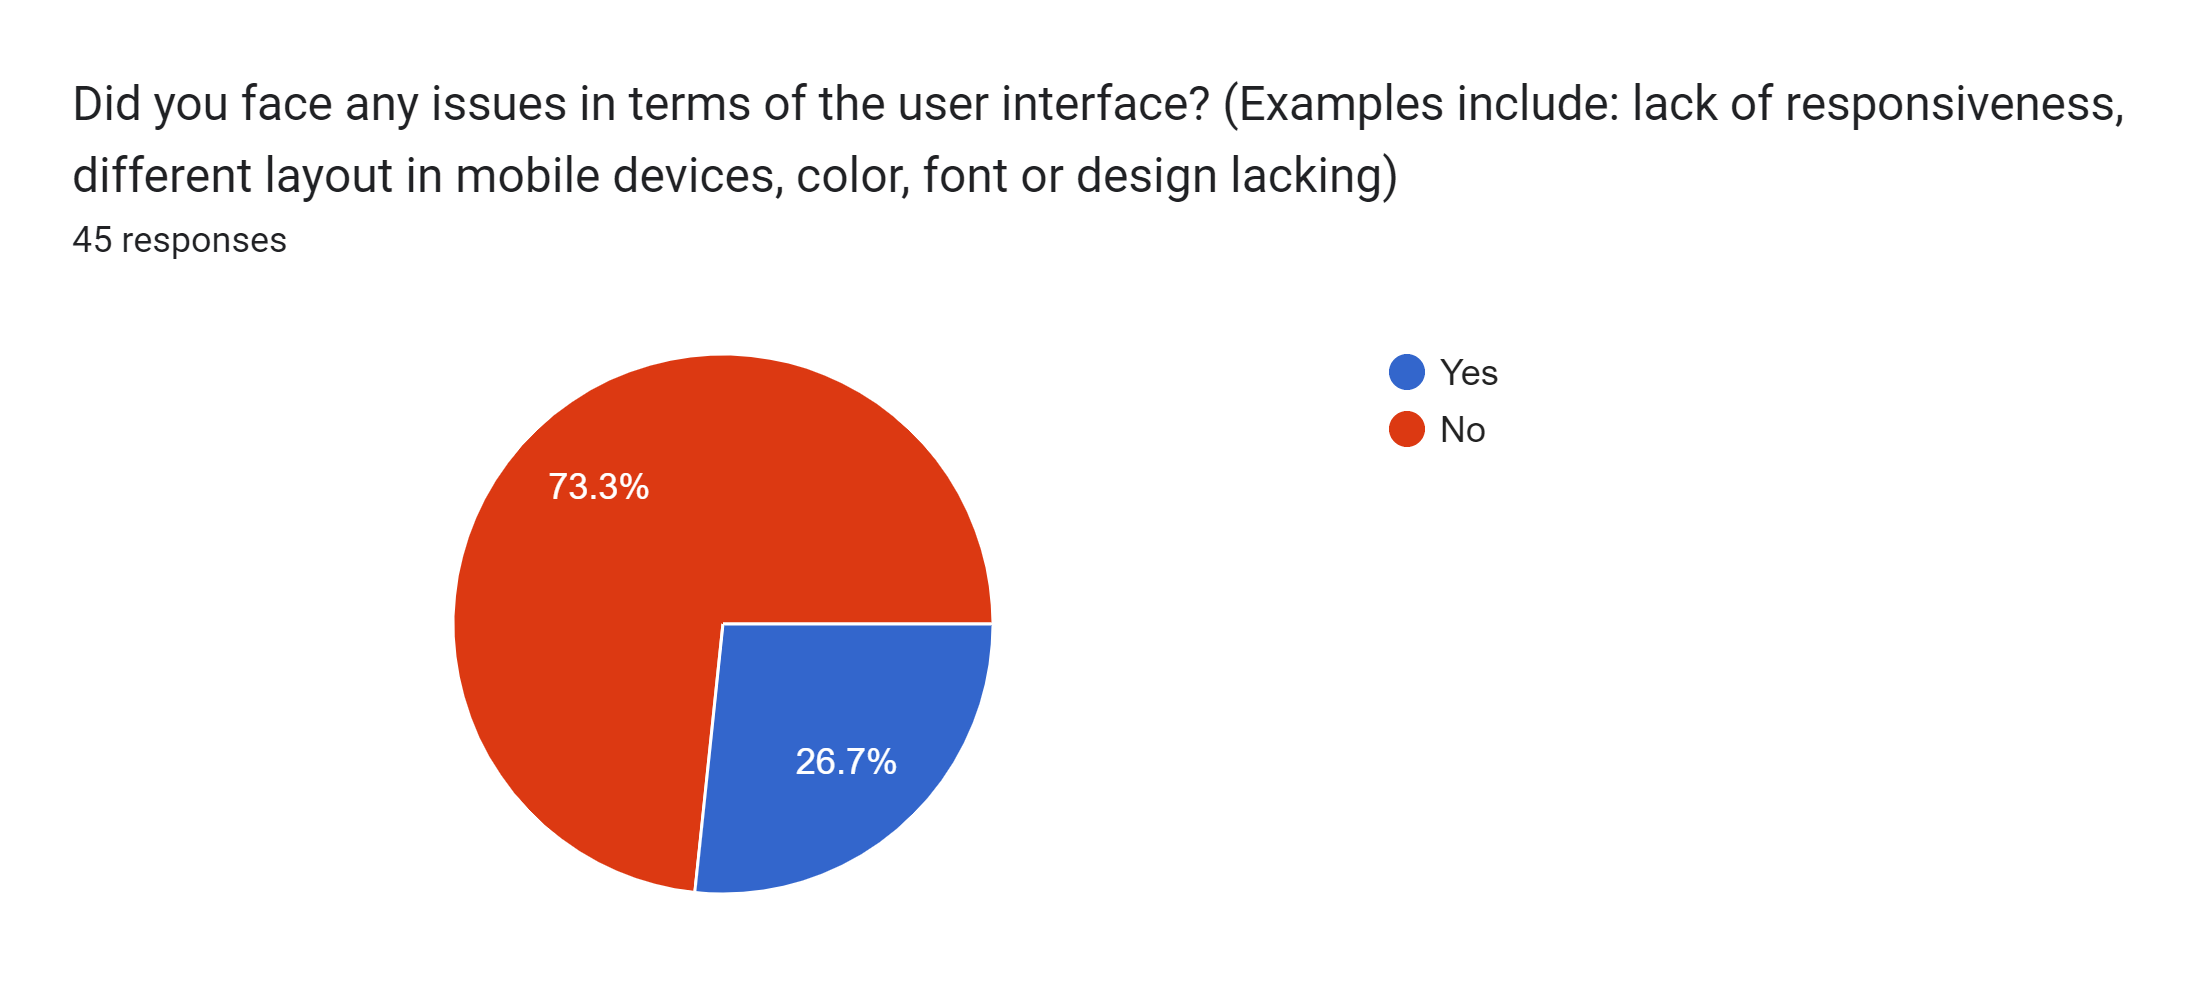
\includegraphics[width=\linewidth]{Figures/issueui.png}}
\vspace{-10pt}\caption{Reason of using e-Passport portal}
\label{fig:issueui}
\end{figure}

\subsubsection{UI Issues} 

The majority of the users shared that they found issues related to UI as pointed out by Fig: \ref{fig:issueui}. Some users faced problems while choosing a suitable interview date. According to their report, while looking for available interview dates, they got their calendar layer completely frozen. Some users let us know that they provided correct and valid information in the form yet got a submission error. Others commented that the UI seemed a bit unorganized, and navigating through the sections was difficult.
\newline

\subsubsection{Technical Issues}

Users had their complaints about the technical side of the website too \ref{fig:issuetech}. A couple of users reported that the 'One Time Password's (OTP) used for prompt verification appeared very late in some cases, hence leading to login and other procedural errors. Some also faced frequent captcha errors. Due to the high amount of system traffic, some of the users got automatically logged out after spending a little time logged in. Available appointment dates were found to be blank in some cases. Moreover, some users suggested that it would be great if there were options to edit or cancel the whole application even after submission in case of emergencies and get refunded, which is not currently available.

\begin{figure}[ht]
\centering
\centerline{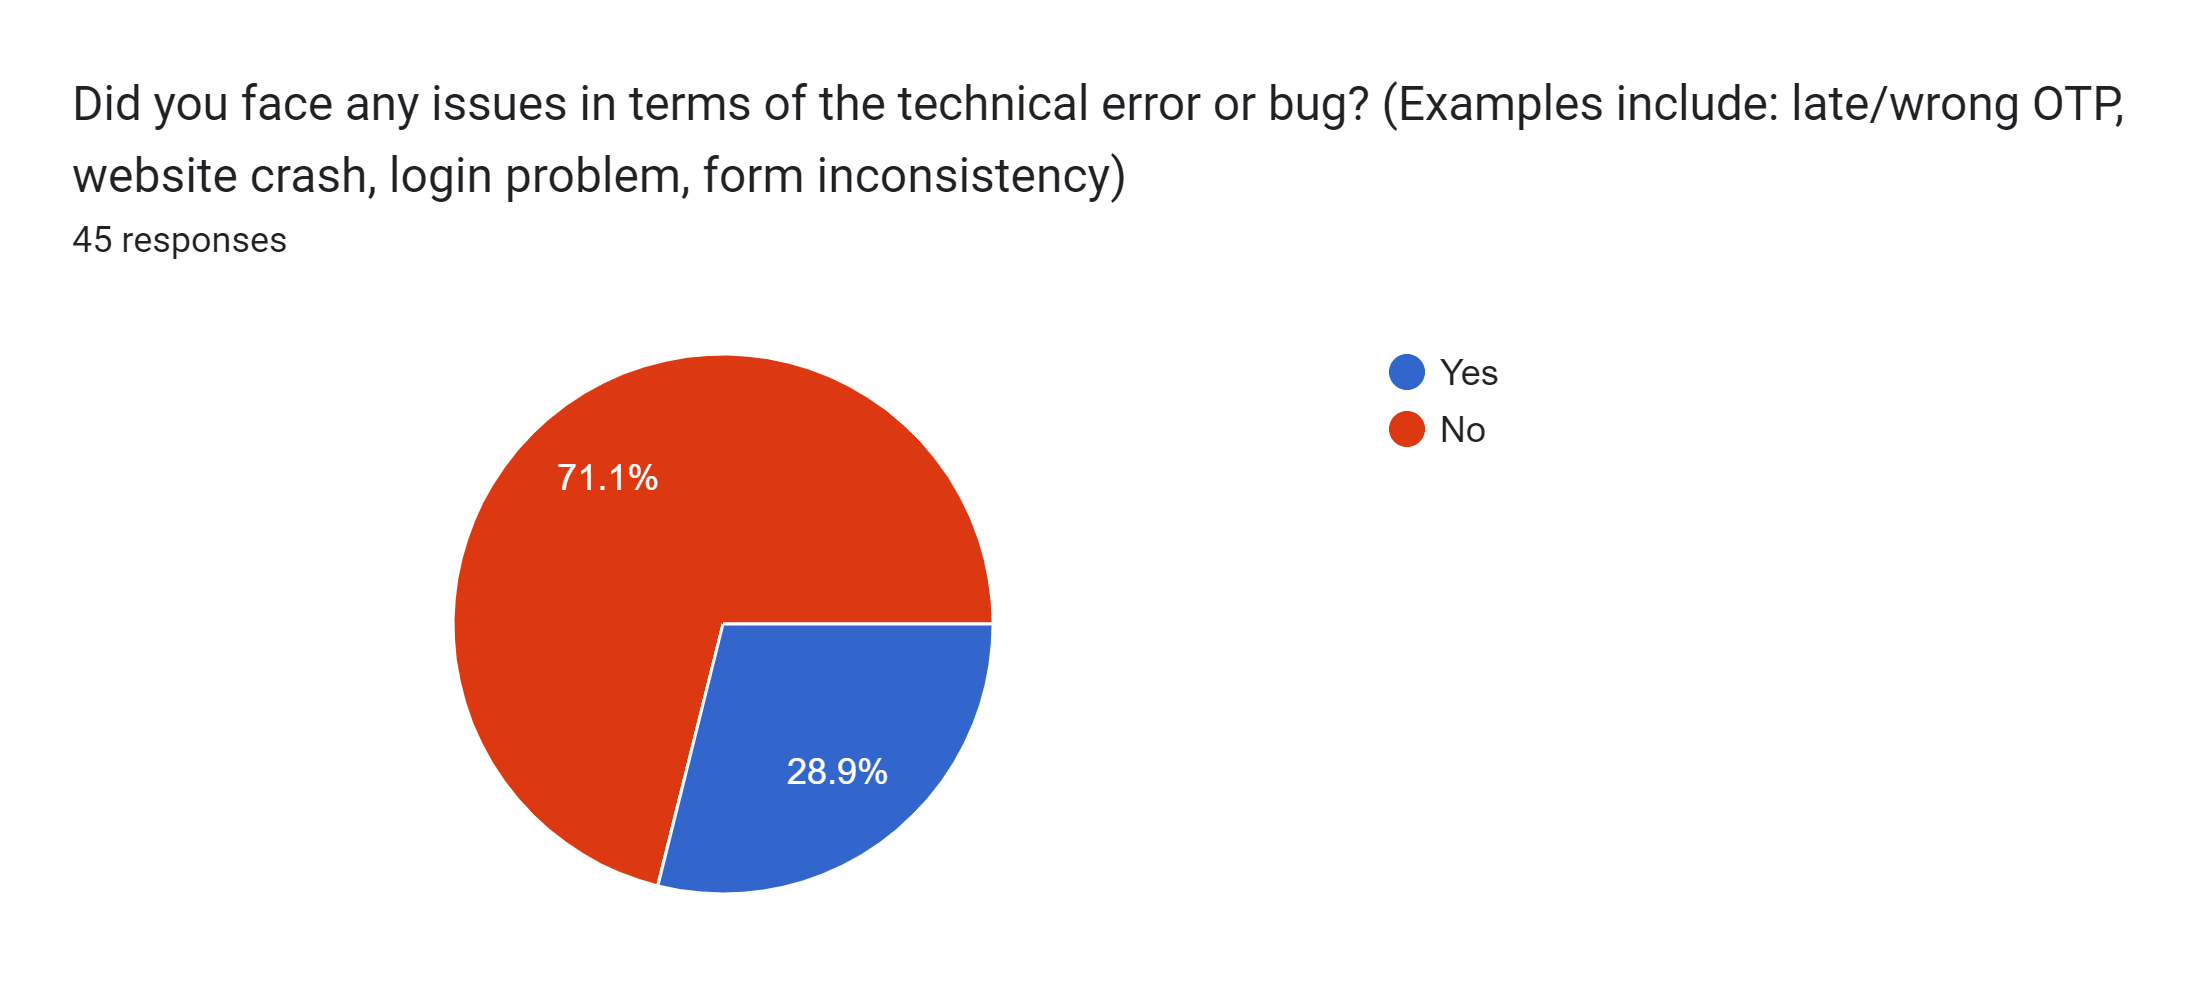
\includegraphics[width=\linewidth]{Figures/issuetech.png}}
\vspace{-10pt}\caption{Percentage of users who faced technical issues}
\label{fig:issuetech}
\end{figure}

A significant portion of the technical complaints was about the online payment system integrated with the website. Around 75.6\% of the users tried to do payments online \ref{fig:payment}, whereas almost 1/6th of the survey attendees mentioned that they could not use the online payment method as the service was down.

\begin{figure}[ht]
\centering
\centerline{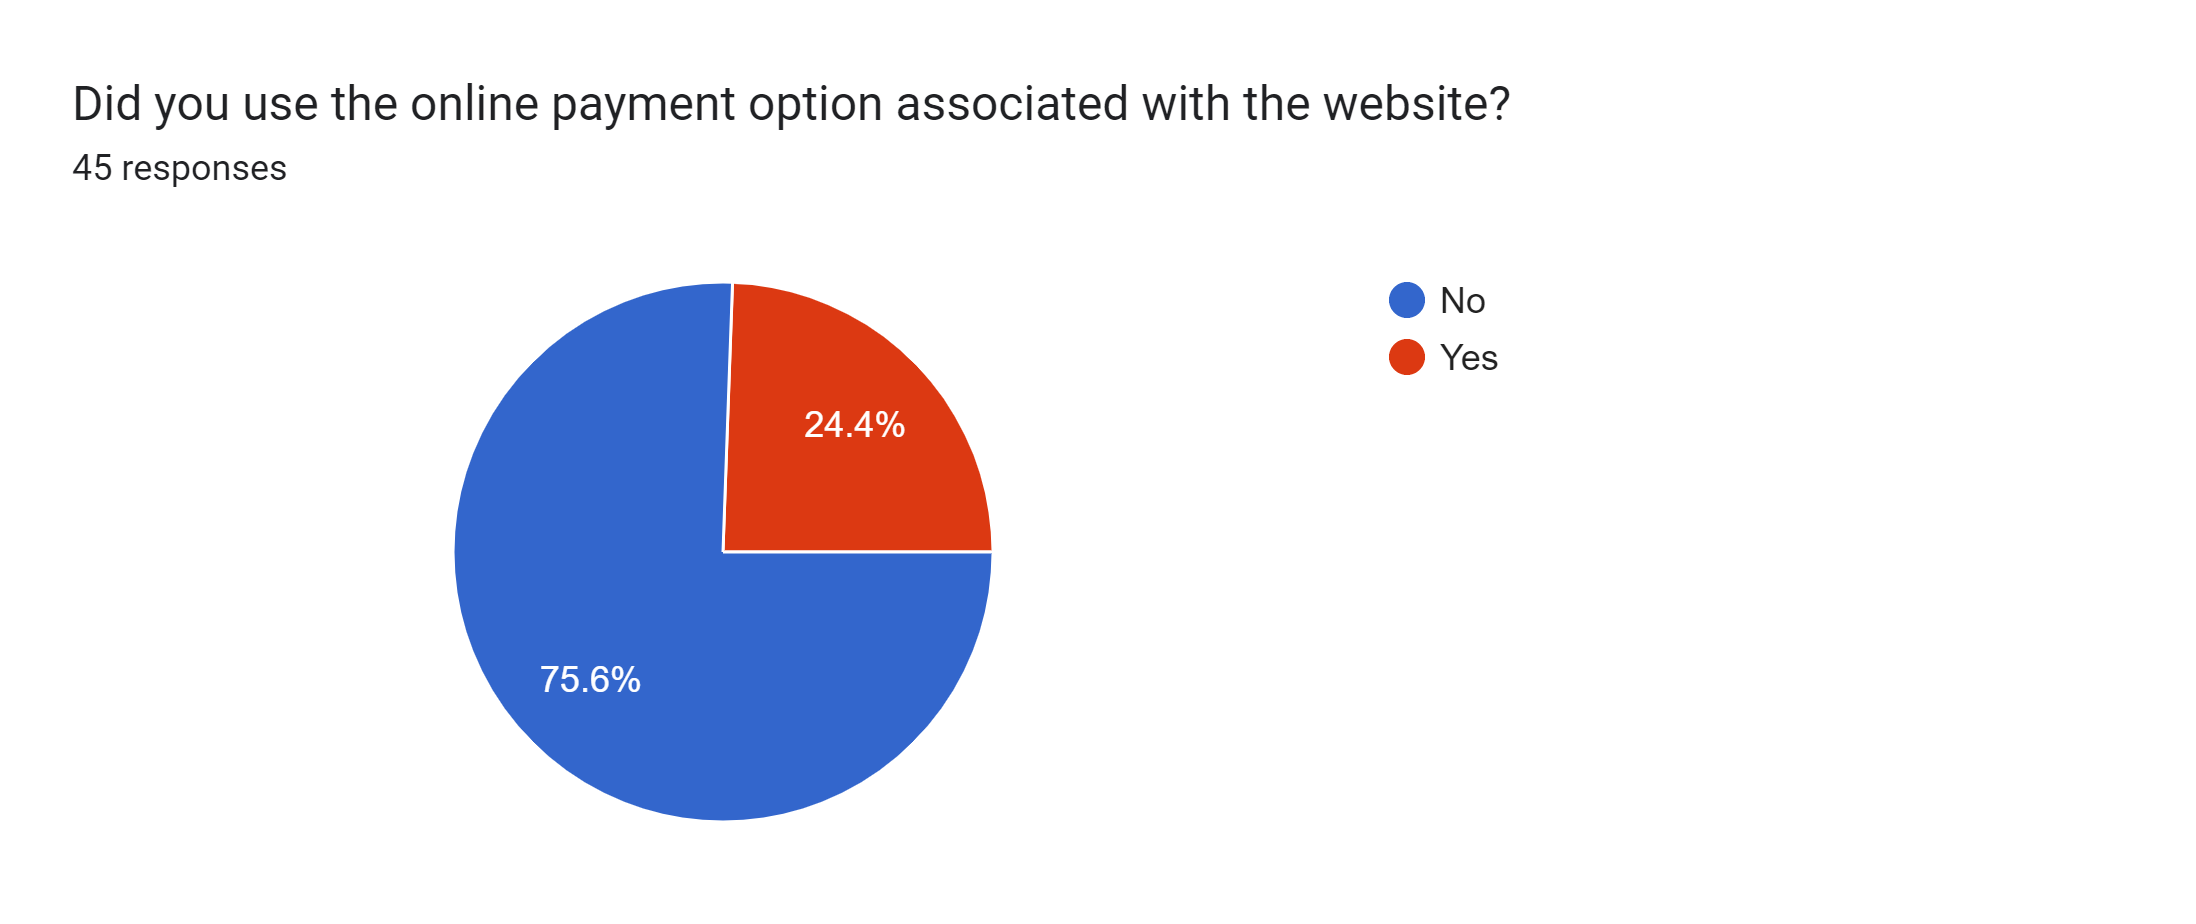
\includegraphics[width=\linewidth]{Figures/payment.png}}
\vspace{-10pt}\caption{Percentage of users who used the online payment module}
\label{fig:payment}
\end{figure}

A couple of clients had to undergo some errors during the payment, but they got their refund as well. One user also mentioned that the current E-Chalan online payment system is far worse than the previous Sonali bank system. The users also reported system crashes and UI freezing during the payment process. Some mentioned that the receipt download option after the confirmation was difficult to find. But apart from these issues, some users also shared that they did not face anything unpleasant while using the online payment.
\newline

\begin{figure}[ht]
\centering
\centerline{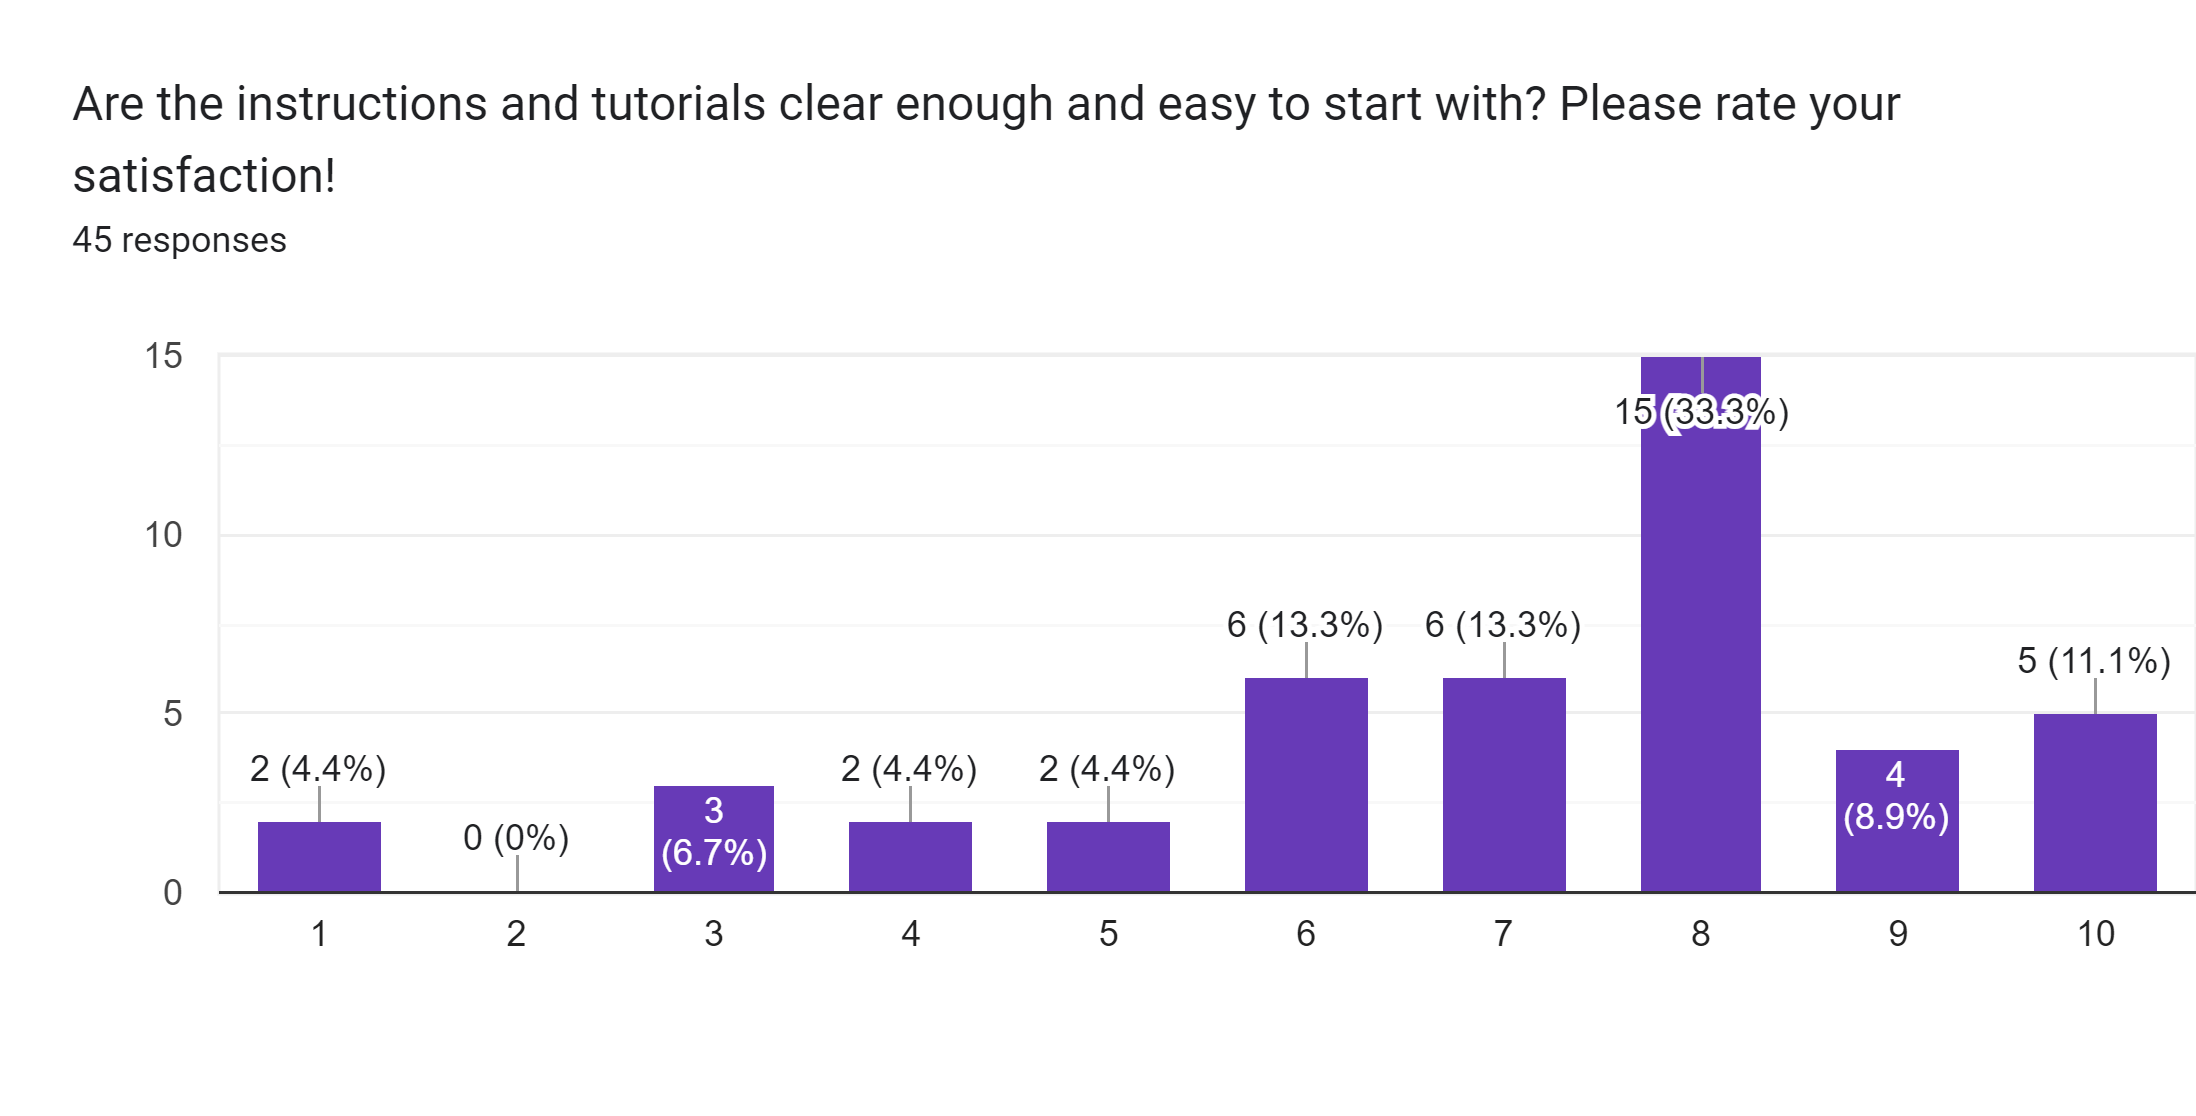
\includegraphics[width=\linewidth]{Figures/instructions.png}}
\vspace{-10pt}\caption{Bar chart showing satisfaction rating in terms of instruction and information clarity}
\label{fig:instruction}
\end{figure}

\subsubsection{Information Gap Issues}

Although most of the users found the information available just fine as per Fig \ref{fig:instruction} and \ref{fig:navigation}, some had their complaints and suggestions as well. The very frequent issue about the information gap the users faced is about no support for punctuation symbols like (.) and (:) in the user full name field. They suggested mentioning this explicitly around the form, otherwise, it was difficult to know whether these symbols were allowed or not. 


\begin{figure}[ht]
\centering
\centerline{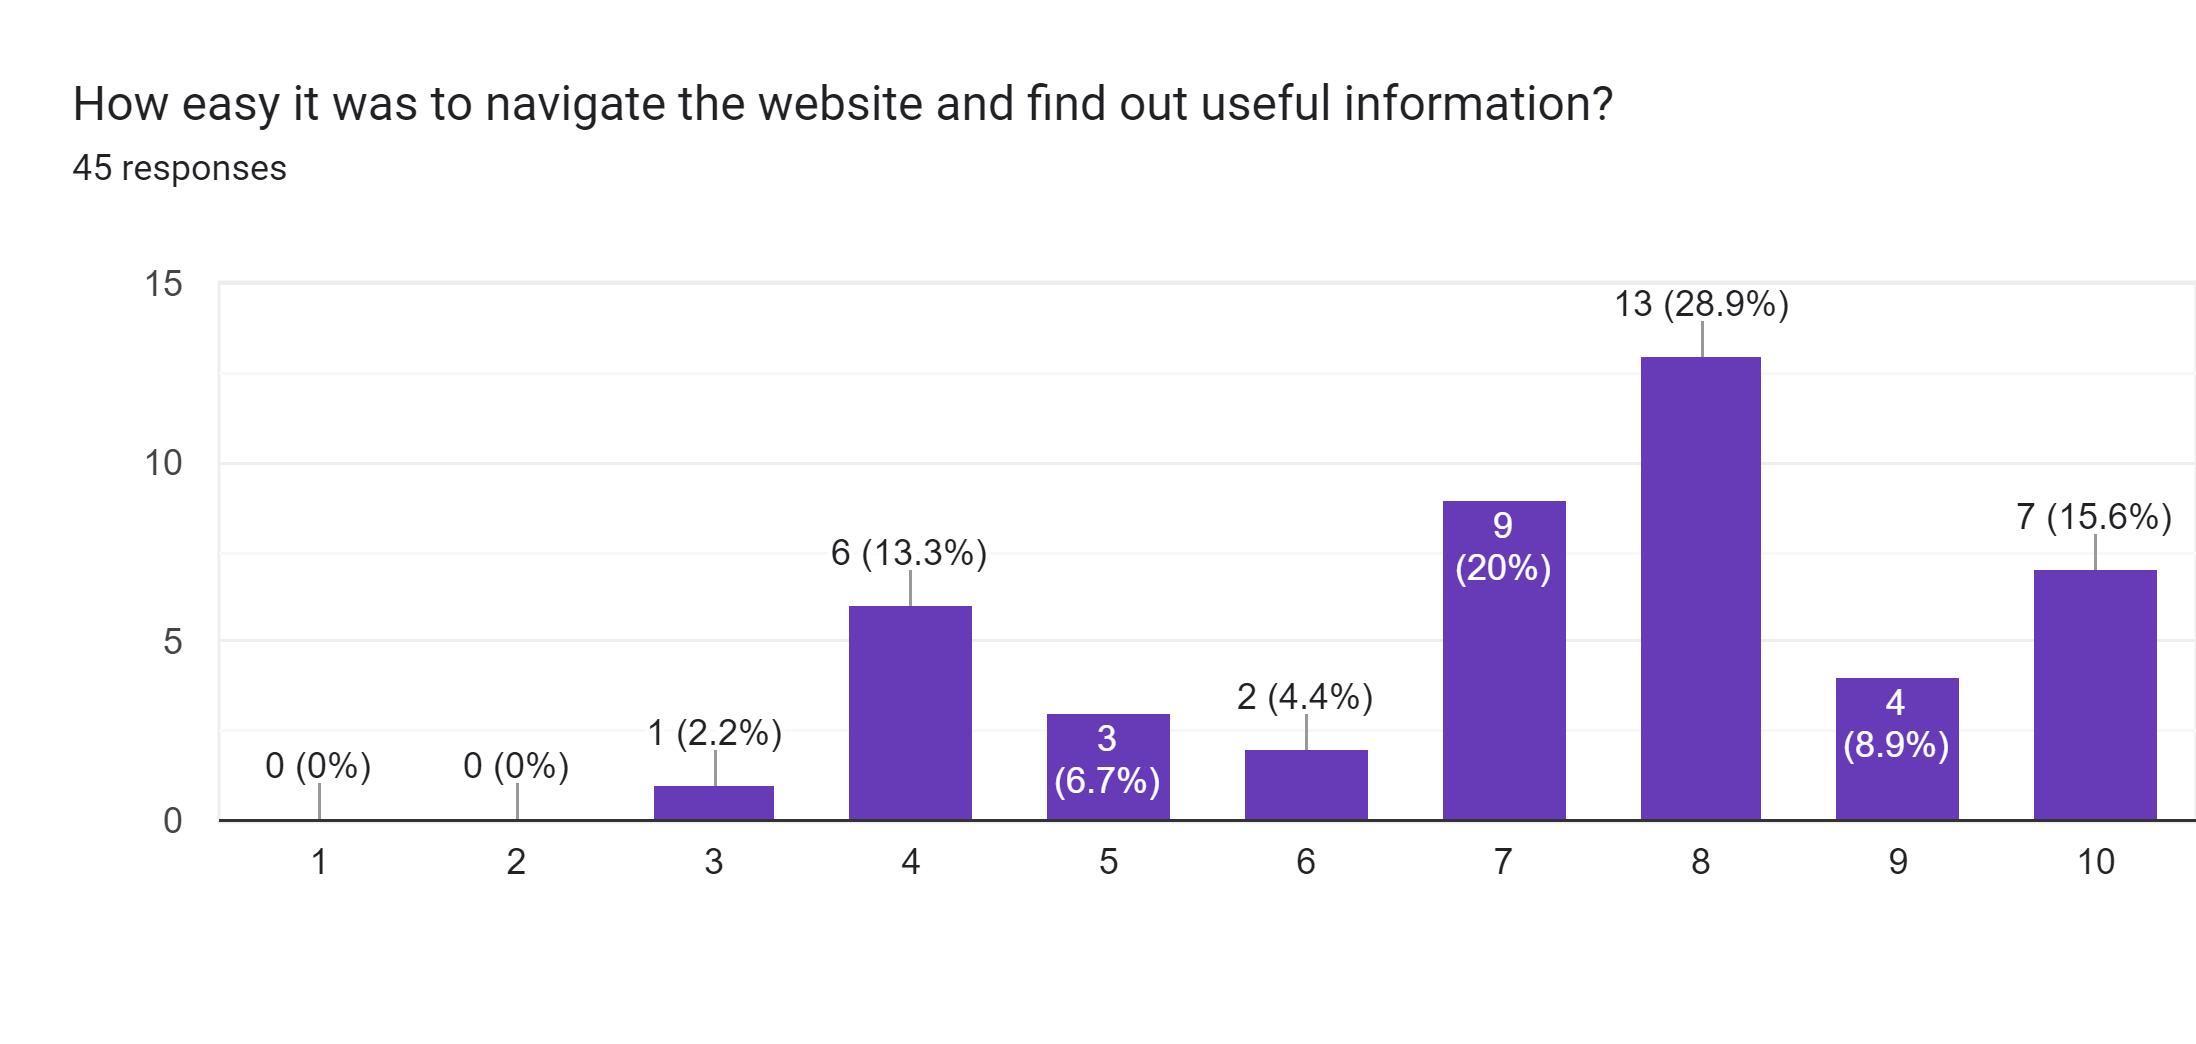
\includegraphics[width=\linewidth]{Figures/navigation.png}}
\vspace{-10pt}\caption{Bar chart showing satisfaction rating in terms of navigation and information}
\label{fig:navigation}
\end{figure}

As we, the authors found out earlier, some users reported that the document list that they needed to bring to the passport office, was not updated and correct on the website, which resulted in nothing but their additional suffering on the due date. Some users mentioned that some video tutorials could be of great help to new users.
\newline

\begin{figure}[ht]
\centering
\centerline{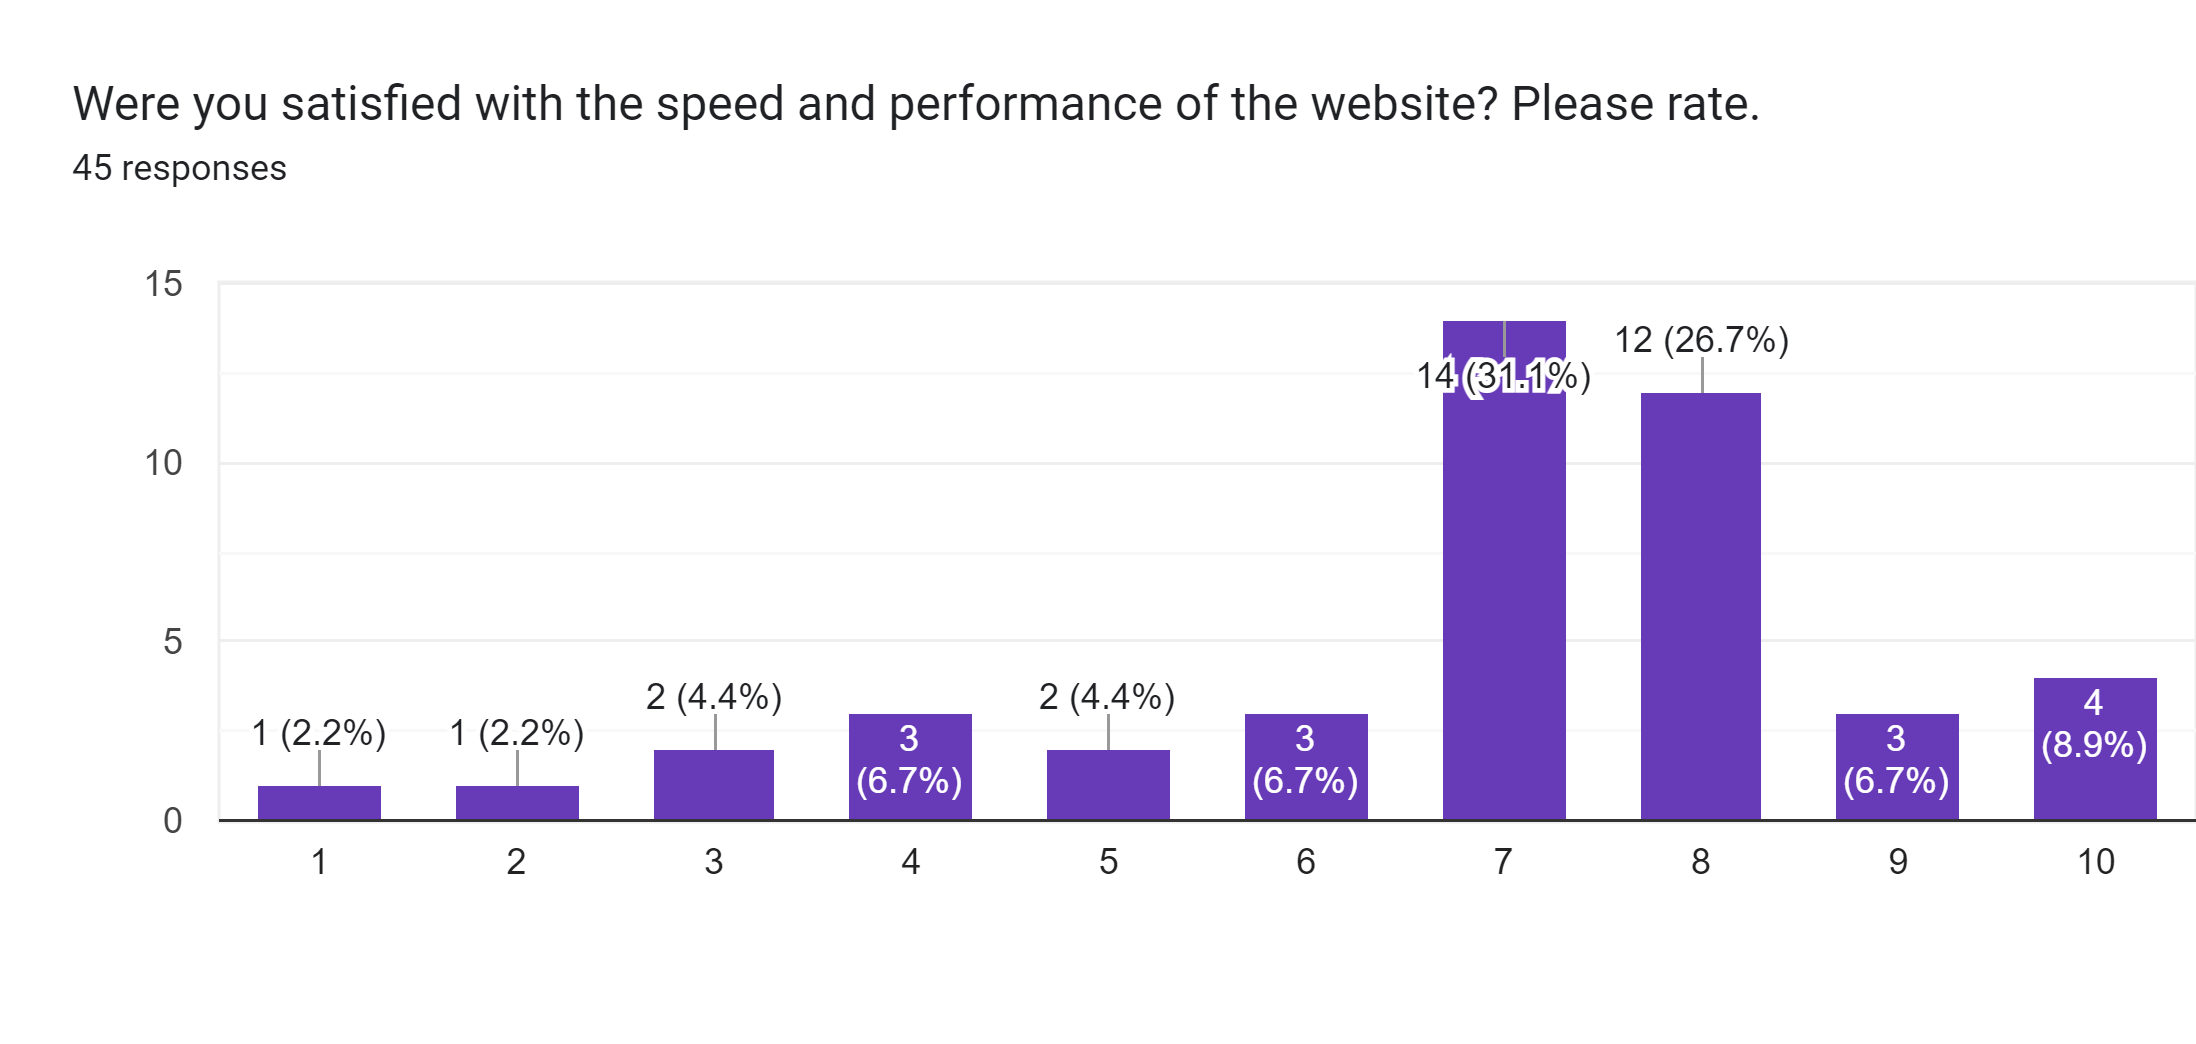
\includegraphics[width=\linewidth]{Figures/speed.png}}
\vspace{-10pt}\caption{Bar chart showing satisfaction rating in terms of speed and performance}
\label{fig:speed}
\end{figure}

\subsubsection{Performance Issues}

As it is quite clear from Fig \ref{fig:speed}, most of the users were quite satisfied with the speed of the software. However, some reported the slow response time of the system. 

Many of the users who already had an expired passport and applied for passport renewal through the website for the first time, shared a common concern. As it should be in a good online system, they were expecting their information to be already present in the database. Users were disappointed to fill up the same information again.
\newline

\subsubsection{Contact and Feedback Services}

Fig \ref{fig:contact} shows that just 13.3\% of the survey takers actually tried these services. Most of the users who tried to use the Contact services for further help reported that the module was not working, and they had to go to the offices physically. Hence, this module showed poor performance just like the payment module mentioned above.
\newline
\begin{figure}[ht]
\centering
\centerline{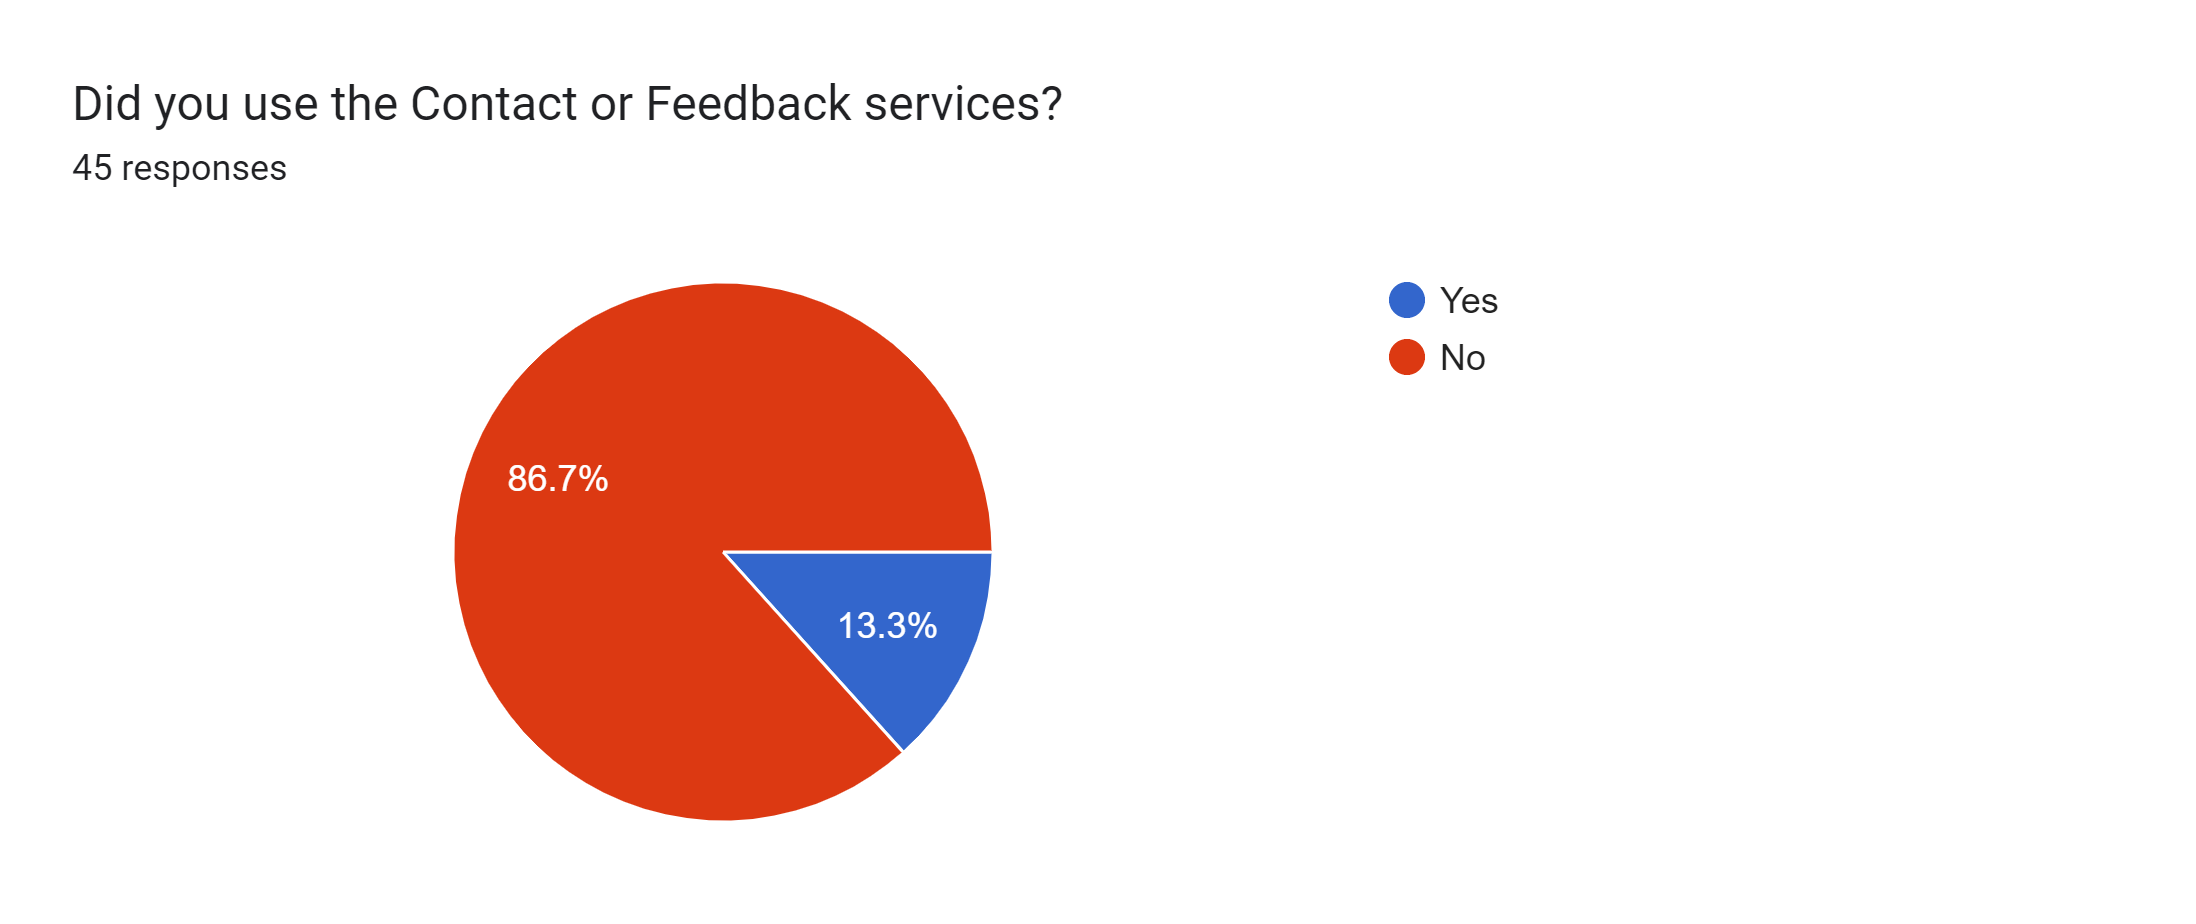
\includegraphics[width=\linewidth]{Figures/contact.png}}
\vspace{-10pt}\caption{Percentage of participants who used Contact or Feedback services}
\label{fig:contact}
\end{figure}

Finally, the users more or less liked the status tracking dashboard of the system as Fig \ref{fig:dash} shows.

\begin{figure}[ht]
\centering
\centerline{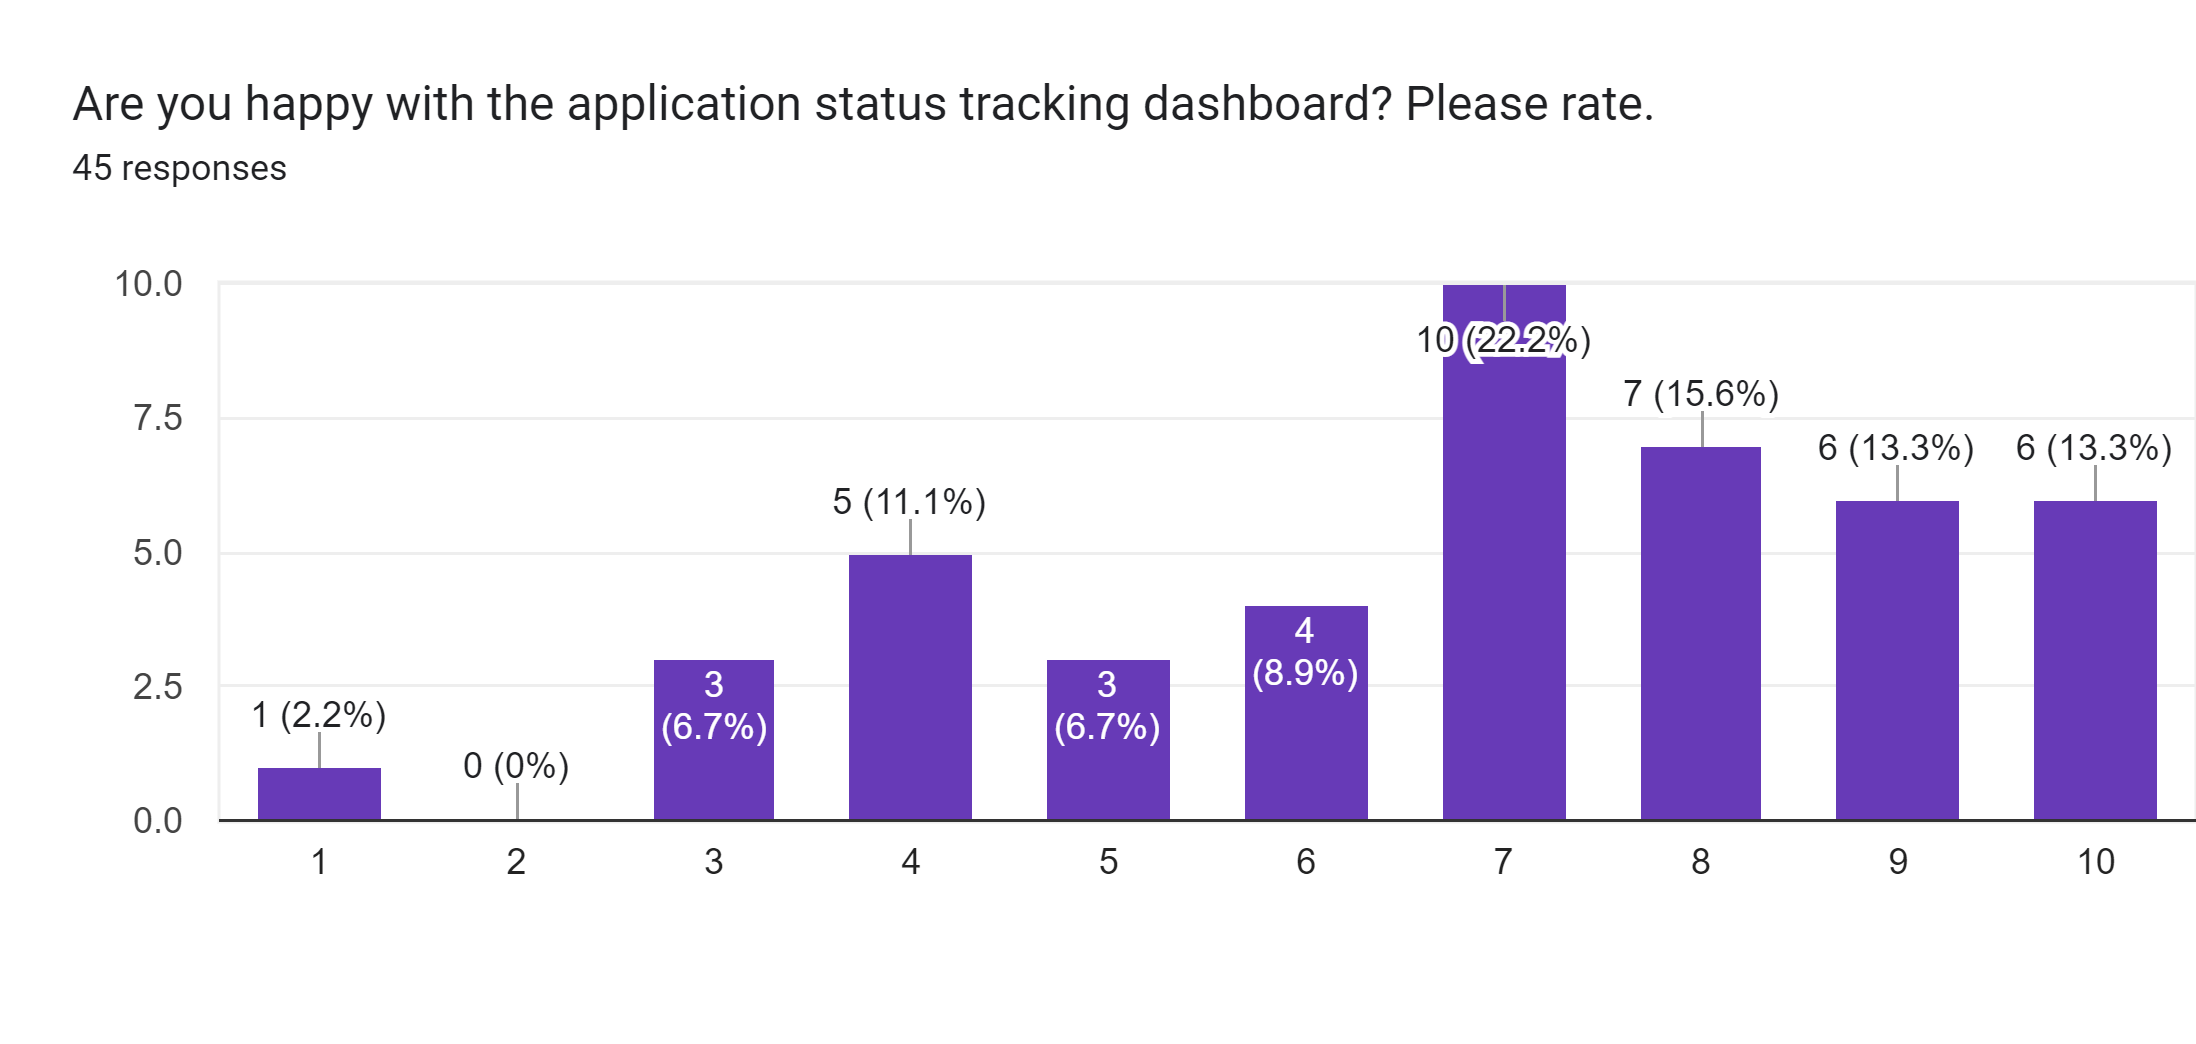
\includegraphics[width=\linewidth]{Figures/dashboard.png}}
\vspace{-10pt}\caption{User satisfaction rating for the application status dashboard}
\label{fig:dash}
\end{figure}

We summarize the positive and negative aspects of the website based on our findings in Table \ref{tab:summary}.

\begin{table*}[ht]
\centering
\caption{Positive and Negative Aspects of Bangladesh e-Passport Portal}
\label{tab:summary}
\begin{tabular}{cll}
\hline
% \begin{table}[ht]
% \begin{tabular}{\columnwidth}{@{\extracolsep{\fill}}}

\textbf{}&\textbf{Positive Aspects} & \textbf{Negative Aspects} \\\hline
1& Serves a huge population & Frequent login, logout and crashing errors\\
2&Status tracking dashboard is handy & Frequent OTP errors \\
3&No major inconsistency issue& Horrible payment module \\
4&Contains system feedback section & Updating, canceling, and refund flexibility needed \\
5&UI components are well-utilized and well-placed& Instructions need to get better \\
6&Offers simple error handling & Complaints about the unresponsiveness of the Contact section\\\hline
\end{tabular}
\end{table*}